\chapter{پیش‌زمینه و کارهای مرتبط‌}
\section{مقدمه}
در این بخش، ابتدا به تبیین مفهوم نوسان و بیان مدل ریاضی آن از دیدگاه‌های متفاوت می‌پردازیم. سپس سعی می‌کنیم تا برخی از کارهای مرتبط در این حوزه را معرفی کنیم. از راهکارهای متفاوتی برای پیش‌بینی‌ سری‌های زمانی مختلف و همچنین نوسان همان سری‌های زمانی استفاده شده است که در ادامه به مطالعه‌ی برخی از ‌آنها خواهیم پرداخت.\\
هرچند به صورت سنتی اکثر مدل‌هاي مربوط به محاسبه‌ي نوسان آماري هستند، فعالیت‌هاي تحقیقاتی متعددي در این زمینه در سالهاي گذشته انجام شده است که دامنه وسیعی از ابزارهاي حوزه هوش مصنوعی را به کار گرفته‌اند. دامنه مجموعه داده‌ي مورد استفاده در این کارها نیز گوناگون است، درحالی که برخی تنها از اطلاعات قیمت و حجم مورد مبادله استفاده می‌کنند، برخی دیگر پا را فراتر گذاشته و از اطلاعات دفتر سفارشات نیز استفاده می‌کنند. برخی دیگر با استفاده از داده‌هاي با فرکانس بسیار بالا و در حد چند میلی‌ثانیه سعی در تخمین وضعیت بازار در بازه‌ی زمانی کوتاهی در آینده را با دقتی بالاتر از حد معمول دارند که در معاملات با فرکانس بالا\LTRfootnote{High-frequency trading} کاربرد دارد. اما تلاش اصلی همواره در جهت به دست آوردن تخمینی از وضعیت بازار در چند دقیقه‌ی آینده در یک بازار مالی بوده‌است.\\
مدل‌های یادگیری عمیق و به ویژه مدل‌های شبکه‌ی عصبی بازگشتی نیز در سال‌های گذشته در زمینه‌ی پیش‌بینی سری‌های زمانی بیشتر به کار گرفته شدند و حتی برخی مطالعات از پیشتازی این روش‌ها در برخی کاربردها خبر می‌دهند.
% از میان این مدل‌ها نیز به معرفی چندگونه خواهیم پرداخت و نحوه‌ی عملکرد ‌آن‌ها را مورد بررسی قرار خواهیم داد.

\section{نوسان} 
در این بخش ابتدا نوسان را به صورت دقیق تعریف می‌کنیم و سپس به مطالعه‌ی تعدادی از مدل‌های نوسانی معروف و نحوه‌ی عملکرد آن‌ها می‌پردازیم.
\subsection{تعریف نوسان}
ابتدا به معرفی نماد‌های مورد استفاده برای تعریف نوسان می‌پردازیم. $P_t$ را قیمت یک دارایی در لحظه‌ی $t$ در نظر می‌گیریم. بازده\LTRfootnote{Return} در لحظه‌ی $t$ به معنای سود یا ضرریست که دارایی مورد نظر در آن لحظه‌ تجربه ‌می‌کند. بر پایه‌ی $P_t$ بازده در لحظه‌ي $t$ به صورت زیر تعریف می‌شود:
\begin{equation}
	\label{eq:t}
	r_t = ln(P_t) - ln(P_{t-1})
\end{equation}
بر این اساس، میانگین بازده در یک پنجره‌ی $N$تایی به صورت زیر تعریف می‌شود:
\begin{equation}
	\label{eq:t1}
		\bar{r}_t = \dfrac{\Sigma_{i=0}^{N-1} r_{t-i}}{N}
\end{equation}
به همین شکل واریانس تغییرات قیمت برای پنجره‌ای به طول $N$، که به عنوان نوسان شناخته می‌شود،‌ به صورت زیر محاسبه می‌شود:
\begin{equation}
	\label{eq:vol}
	v_t = \sqrt{\dfrac{\Sigma_{i=0}^{N-1} (r_{t-i}-\bar{r})^2}{N}}
\end{equation}
طبق رابطه‌ی بالا می‌توان سری زمانی نوسان، $v_t$ را در طول زمان تشکیل داد.
\section{مدل‌های نوسانی}
در ادامه به معرفی ویژگی‌های مدل‌های نوسانی مختلف و بررسی نحوه‌ی کارکرد برخی از آن‌ها می‌پردازیم. مطالعات پیشین به استفاده و بررسی گسترده از مدل‌های بر پایه‌ی مدل گارچ\LTRfootnote{GARCH} برای پیش‌بینی نوسان پرداخته اند\cite{katsiampa2017volatility}و\cite{liu2019volatility}. برخی دیگر از روش‌های مبتنی بر مدل‌های احتمالاتی گرافی برای استفاده از اطلاعات موجود در دفتر سفارشات استفاده کرده‌اند\cite{guo2018bitcoin}.\\
\subsection{مدل‌های گارچ}
برای درک نحوه‌ی کارکرد مدل‌های گارچ ابتدا باید از گونه‌ی ساده تری از مدل ها به نام آریما\LTRfootnote{Arima} که خود شامل سه بخش کاهنده‌ی خودکار\LTRfootnote{Auto Regressive}، میانگین متحرک\LTRfootnote{Moving Average} و بخش تجمعی\LTRfootnote{Integrated} هستند شروع کنیم.
\subsubsection{مدل‌های کاهنده‌ی خودکار}
$AR(p)$ یک مدل کاهنده‌ی خودکار از مرتبه‌ی $p$ است که از پس‌افت‌های\LTRfootnote{Lag} سری زمانی اصلی به عنوان متغیرهای پیش‌بینی همان سری زمانی در آینده استفاده می‌کند. مقدار $p$  بیان کننده‌ی مرتبه‌ی مدل است. به عنوان مثال، $AR(1)$ از پس‌افت اول سری زمانی، یعنی $x_{t-1}$، برای پیش بینی $x_t$ استفاده می‌کند. بنابراین می‌توان  یک مدل کاهنده‌ی خودکار  از مرتبه‌ی $p$را به صورت زیر تعریف کرد\cite{ariyo2014stock}:
\begin{equation}
	x_t = \phi_0 + \phi_1 x_{t-1} + \phi_2 x_{t-2} + ... + \phi_p x_{t-p} + \epsilon_t
\end{equation}
که $\epsilon_t$ در آن نویز سفید\LTRfootnote{White Noise} است. در واقع $\epsilon$ هربار بعد از مشاهده‌ی مقدار اصلی سری زمانی به صورت اختلاف پیش‌بینی مدل و مقدار اصلی محاسبه می‌شود. $\epsilon$ در حالت ایده‌آل نویز سفید است، چرا که در این صورت می‌توانیم مطمئن باشیم که مدل تمامی الگوهای موجود در سری زمانی را مدل کرده است و مقدار باقیمانده\LTRfootnote{Residual Value} از سری‌زمانی کاملا تصادفی و غیرقابل مدل کردن است.

\subsubsection{مدل‌های میانگین متحرک}
این مدل‌‌ها از جهاتی به مدل‌های کاهنده‌ی خودکار شبیه هستند، اما به جای استفاده از پس‌افت‌های قبلی سری زمانی،‌ از خطاها($\epsilon$) برای پیش‌بینی استفاده می‌کنند. مدل‌ $MA(q)$ یک مدل‌ میانگین متحرک از مرتبه‌ی $q$ است که از تعداد $q$ خطای قبلی برای پیش‌بینی سری زمانی استفاده می‌کند، که به صورت زیر تعریف می‌شود:
\begin{equation}
	x_t = \epsilon_t + \theta_1 \epsilon_{t-1} + \theta_2 \epsilon_{t-2} + ... + \theta_q \epsilon_{t-q} + \mu
\end{equation}
که $\mu$ بیانگر میانگین ثابت است.
\subsubsection{مدل‌های آریما}
این مدل‌های که به نوعی ترکیب دو مدل قبلی هستند، از تمامی ویژگی‌های موجود در آن‌ها بهره می‌برند. این مدل‌ها ابتدا متغیر جدید $y_t$ را به صورت زیر تعریف می‌کنند:
\begin{equation}
	\label{eq:airami}
	y_t = x_t - x_{t-1}
\end{equation}
علت تعریف $y_t$  به این صورت از بین بردن رشد خطی یک سری زمانی یا روند سیر\LTRfootnote{Trend} آن است. بدیهی است که در صورت توانایی پیش‌بینی سری‌زمانی $y$ می‌توان به راحتی سری زمانی $x$ را با داشتن یک مقدار اولیه به دست آورد. مدل آریما سری زمانی $y_t$ را به صورت زیر مدل می‌کند:
\begin{equation}
	\label{eq:arimapq}
	y_t = \phi_0 + \phi_1 x_{t-1} + ... + \phi_p x{t-p} + \epsilon_t + \theta_1 \epsilon_{t-1} + ... + \theta_q \epsilon_{t-q}
\end{equation}
که مانند مدل‌های قبلی مقادیر $p$ و $q$ مرتبه‌ی مدل آریما را مشخص می‌کنند. $p$ مرتبه‌ی قسمت کاهنده‌ی خودکار و $q$ مرتبه‌ی قسمت میانگین متحرک است. مدل‌ پارامتر دیگری به نام $i$ نیز دارد که عموما مقدار ۱ دارد اما بسته به کاربرد ممکن است تغییر کند و مقداری بیشتر از ۱ بگیرد. $i$ در مدل آریما مشخص می‌کند که عمل تفاضل‌گیری از سیگنال اولیه چندبار انجام شود. به عنوان مثال، رابطه‌ی \ref{eq:airami} نشان‌دهنده‌ی یکبار تفاضل‌گیری از سیگنال اولیه است. در صورتی که $i$ مقداری بیشتر از یک داشته باشد، باید عمل تفاضل‌گیری برای $y_t$ نیز تکرار شود تا سری زمانی جدید تشکیل شود و سپس از رابطه‌ی \ref{eq:arimapq} برای مدل‌کردن آن استفاده شود.
\subsubsection{مدل‌های آرچ}
مدل‌های بر پایه‌ی آرچ\LTRfootnote{Autoregressive conditional heteroskedasticity} با تمرکز بر پیش‌بینی نوسان به وجود آمده‌اند. این مدل میزان نوسان هر نقطه‌ی زمانی را با استفاده از خطای پیش‌بینی در نقاط قبل از آن یعنی $\epsilon$ها مدل‌ می‌کند. این مدل نیز مانند مدل‌های پیشین برای پایه‌های مختلف تعریف می‌شود. تعریف یک مدل آرچ به ازای پایه‌ی $r$ برابرست با:
\begin{equation}
	\epsilon_t = w_t \sqrt{\alpha_0 + \alpha_1 \epsilon_{t-1}^2 + \alpha_2 \epsilon_{t-2}^2 + ... + \alpha_r \epsilon_{t-r}^2}
\end{equation}
که در حالت ایده‌آل، $w_t$ در آن باید نویز سفید باشد که بعد از مشاهده‌ی مقدار اصلی نوسان دنباله‌ی هدف قابل محاسبه می‌باشد.
\subsubsection{مدل‌های گارچ}
نحوه‌ی بدست آمدن مدل‌ گارچ از روی مدل‌ آرچ بسیار شبیه به روند تبدیل مدل‌ کاهشی خودکار به آریماست. در تبدیل مدل کاهشی خودکار به آریما شاهد بودیم که با اضافه کردن یک مجموعه متغیر جدید که نشان‌دهنده‌ی خطای پیش‌بینی‌های گذشته بودند، مدل‌ کامل‌تری ساخته شد که می‌توانست از خطاهای قبلی خود در جهت بهبود پیش‌بینی‌های بعدی استفاده کند. در تبدیل آرچ به گارچ نیز با اضافه کردن پس‌افت‌های خود سری زمانی نوسان به مدل قبلی،‌ می‌توانیم دنباله‌های بیشتری را مدل کنیم. رابطه‌ی گارچ برای پایه‌های $p$ و $q$ به صورت زیر است:
\begin{equation}
	\label{garch:one}
	\epsilon_t = w_t \sqrt{\alpha_0 + \alpha_1 \epsilon_{t-1}^2 + ... + \alpha_p \epsilon_{t-p}^2 + \beta_1 \delta_{t-1}^2 + ... + \beta_q \delta_{t-q}^2}
\end{equation}
در تعریف بالا $\delta_{t}$ به معنای نوسان در لحظه‌ی $t$ است که به صورت زیر قابل محاسبه است:
\begin{equation}
	\label{garch:twol}
	\delta_t = \sqrt{\alpha_0 + \alpha_1 \epsilon_{t-1}^2 + \alpha_2 \epsilon_{t-2}^2 + ... + \alpha_q \epsilon_{t-q}^2}
\end{equation}
با استفاده از \ref{garch:one} و \ref{garch:twol} می‌توان رابطه‌ی گارچ را به صورت زیر بازنویسی کرد:
\begin{equation}
	\epsilon_t = w_t \sqrt{\delta_{t} + \beta_1 \delta_{t-1}^2 + ... + \beta_q \delta{t-q}^2}
\end{equation}
که مانند مدل‌های قبلی $w_t$ نویز سفید است.
\subsection{دفتر سفارشات}
در این بخش به مطالعه‌ی بخشی از مطالعات انجام شده بر روی اطلاعات دفتر سفارشات خواهیم پرداخت. ابتدا به معرفی ساختار دفتر سفارشات خواهیم پرداخت و سپس مشاهده‌ خواهیم کرد که این داده ساختار چگونه اطلاعات مربوط به وضعیت بازار و سفارشات را در خود جای می‌دهد. در ادامه به بررسی چند نمونه از مطالعات انجام شده بر روی دفتر سفارشات خواهیم پرداخت و با اهمیت این داده ساختار در مطالعه‌ی بازارهای مالی آشنا خواهیم شد.
\begin{figure}[!t]
	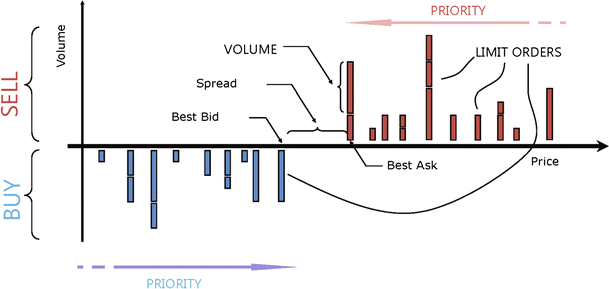
\includegraphics[width=1.0 \textwidth]{images/orderbook_1}
	\centering
	\caption{ نمودار ساختار دفتر سفارشات به همراه برخی ویژگی‌های مربوط\cite{brabazon2016characterising}.
	}
	\label{fig.orderbook_1}
\end{figure}

\subsubsection{ساختار دفتر سفارشات}
به طور خلاصه دفتر سفارشات شامل تمامی سفارش‌های خرید و فروش در جریان در یک بازار مالی و مربوط به یک دارایی مشخص است. این دفتر شامل سفارشات به صورت یک دوتایی مرتب شامل قیمت و حجم متناظر است. تمام سفارش‌هایی که دارای قیمت یکسانی باشند با یکدیگر تجمیع می‌شوند و به صورت یک دوتایی مرتب با همان قیمت و مجموع حجم همه‌ی آن‌ها در دفتر ثبت می‌شوند.\\
این دوتایی‌های مرتب را می‌توان بر اساس قیمت مرتب کرد تا بتوان ترتیبی برای نحوه‌ی جور کردن آن‌ها در جریان فعالیت بازار در نظر گرفت. در صورت مرتب‌سازی این دوتایی‌ها بر اساس قیمت، مانند شکل \ref{fig.orderbook_1}، شاهد جداسازی سفارش های مربوط به خرید و سفارش‌های مربوط به فروش خواهیم بود. علت این امر آن است که سفارش‌های خرید همواره قیمت کمتری نسبت به قیمت سفارش‌های موجود برای فروش دارند، زیرا که اگر چنین نبود سفارش خرید به محض ایجاد با یک سفارش فروش متناظر می‌شد و معامله‌ انجام می‌شد و هر دو سفارش از دفتر سفارشات خارج می‌شدند.\\
سپس در حالی که دوتایی‌ها بر اساس قیمت مرتب‌سازی شده‌اند می‌توان یک ترتیب ‌برای نحوه‌ی جورسازی و اجرای آن‌ها در نظر گرفت. سفارش‌های فروش به ترتیب از قیمت کم به زیاد دارای اولویت زیاد به کم هستند چرا که خریداران همواره تمایل به خرید یک دارایی با کمترین قیمت ممکن را دارند و در نتیجه اگر قیمت پیشنهادیشان بیشتر از چند سفارش فروش مختلف باشد،‌ اقدام به خرید از ارزان‌ترین آن‌ها می‌کنند. برعکس همین مسئله برای سفارش‌های خرید برقرار است. بدین ترتیب سفارشی که بیشترین میزان قیمت پیشنهادی را داشته باشد از بالاترین اولویت برخوردار است و در صورتی که سفارش فروش جدیدی با قیمتی کمتر از چند سفارش خرید موجود در بازار ایجاد شود،‌ به طور خودکار با گران‌ترین سفارش خرید جور شده و اجرا می‌شود.\\
از طرف دیگر ویژگی‌های دیگری نیز در دفتر سفارشات وجود دارد که مورد علاقه‌ی تحلیلگران و فعالین این حوزه بوده است. از مهم ترین آن‌ها می‌توان به شکاف قیمت\LTRfootnote{Spread} که در شکل \ref{fig.orderbook_1} نیز مشاهده می‌شود اشاره کرد. شکاف قیمت بیانگر اختلاف موجود بین ارزان‌ترین پیشنهاد فروش و گران‌ترین پیشنهاد خرید است. به طور معمول افزایش میزان شکاف قیمتی خبر از اختلاف میان خریداران و فروشندگان می‌دهد که می‌تواند باعث افزایش یا کاهش شدید قیمت در آینده‌ی نزدیک بشود که در هر دو حالت با افزایش نوسان همراه خواهد بود.\\
در مطالعه‌ای نشان داده شده است که با استفاده از ویژگی‌های مختلف دفتر سفارشات می‌توان نوسان را با دقت بیشتری نسبت به روش‌هایی که ازین اطلاعات استفاده نمی‌کنند تخمین زد\cite{guo2018bitcoin}. این مقاله با استفاده از یک مدل احتمالاتی گرافی و اطلاعات دفتر سفارشات، موفق شده است که نوسان را با دقت بیشتری نسبت به مدل‌های گارچ پیش‌بینی کند. همچنین نکته‌ی دیگری که در این مقاله‌ حائز اهمیت است، مقایسه‌ی نتایج نهایی به دست آمده توسط این مدل با مدل‌های ساده‌ی شبکه‌ی عصبی است که نشان دهنده‌ی برتری شبکه‌های عصبی در برخی بازه‌های زمانی نیز هست.
\subsection{جمع بندی}
در این فصل با برخی روش‌های آماری برای پیش‌بینی سری‌های زمانی و نوسان آن‌ها آشنا شدیم. سپس به بررسی و معرفی دقیق‌تر دفتر سفارشات پرداختیم.
% و در انتها با روش‌های مبتی بر شبکه‌های عصبی برای محاسبه‌ی سری‌های زمانی آشنا شدیم.


